\documentclass[conference]{IEEEtran}
\IEEEoverridecommandlockouts

\usepackage{cite}
\usepackage{amsmath,amssymb,amsfonts}
\usepackage{graphicx}
\usepackage{array}
\usepackage{booktabs}
\usepackage{textcomp}
\usepackage[hidelinks]{hyperref}
\graphicspath{{figs/}}

% Generated by make_numbers.py from the locked run artifacts.
% AUTO-GENERATED by make_numbers.py -- do not edit by hand.
% Sources (locked, read-only):
%   artifacts/locked_results/verified_v1_20260521_173612_CEST
%   artifacts/paper_handoff_20260603/off_system_eval_summary.csv

\newcommand{\AbstainShareLINC}{78}
\newcommand{\AbstainShareLogicLM}{3}
\newcommand{\AbstainShareLongCtx}{0}
\newcommand{\AccLINC}{94.88}
\newcommand{\AccLINCLogic}{95.36}
\newcommand{\AccLINCOpen}{91.62}
\newcommand{\AccLINCRecall}{95.45}
\newcommand{\AccLeastRuleLongCtx}{97.75}
\newcommand{\AccLogicLM}{96.99}
\newcommand{\AccLogicLMLogic}{93.62}
\newcommand{\AccLogicLMOpen}{97.82}
\newcommand{\AccLogicLMRecall}{99.96}
\newcommand{\AccLongCtx}{96.57}
\newcommand{\AccLongCtxLogic}{93.09}
\newcommand{\AccLongCtxOpen}{96.56}
\newcommand{\AccLongCtxRecall}{99.93}
\newcommand{\AccMostRuleLongCtx}{93.70}
\newcommand{\AccSys}{100.00}
\newcommand{\AccSysLogic}{100.00}
\newcommand{\AccSysOpen}{100.00}
\newcommand{\AccSysRecall}{100.00}
\newcommand{\BaseBestLogic}{95.36}
\newcommand{\BaseBestOpen}{97.82}
\newcommand{\BaseBestRecall}{99.96}
\newcommand{\BaseWorstLogic}{93.09}
\newcommand{\BaseWorstOpen}{91.62}
\newcommand{\BaseWorstRecall}{95.45}
\newcommand{\BestAtLogic}{LINC}
\newcommand{\BestAtOpen}{LogicLM}
\newcommand{\BestAtRecall}{LogicLM}
\newcommand{\CleanLINCLogic}{99.88}
\newcommand{\CleanLogicLMLogic}{99.39}
\newcommand{\CleanLongCtxLogic}{98.99}
\newcommand{\CompLogic}{1.00}
\newcommand{\CompMaxLogic}{1}
\newcommand{\CompMaxOpen}{6}
\newcommand{\CompMaxRecall}{7}
\newcommand{\CompOpen}{1.71}
\newcommand{\CompRecall}{1.02}
\newcommand{\DerivMax}{3}
\newcommand{\DerivMin}{1}
\newcommand{\DiscBaselineOnlyMax}{0}
\newcommand{\DiscLINCBaseOnly}{0}
\newcommand{\DiscLINCSysOnly}{321}
\newcommand{\DiscLogicLMBaseOnly}{0}
\newcommand{\DiscLogicLMSysOnly}{189}
\newcommand{\DiscLongCtxBaseOnly}{0}
\newcommand{\DiscLongCtxSysOnly}{215}
\newcommand{\DocCompoundPctOpen}{38}
\newcommand{\DocCompoundPctRec}{19}
\newcommand{\DocGoldCharsOpen}{29.8}
\newcommand{\DocGoldCharsRec}{19.5}
\newcommand{\DomainAgreeMin}{100}
\newcommand{\DomainLeastRule}{viessmann}
\newcommand{\DomainMostRule}{battery}
\newcommand{\DomainOrdering}{monotone}
\newcommand{\EmbedModel}{\texttt{all-MiniLM-L6-v2}}
\newcommand{\ErrLINC}{321}
\newcommand{\ErrLogicLM}{189}
\newcommand{\ErrLongCtx}{215}
\newcommand{\ErrSys}{0}
\newcommand{\ExcludedReasons}{8}
\newcommand{\ExcludedRows}{645}
\newcommand{\GenModel}{\texttt{gpt-4o-mini}}
\newcommand{\HeadroomLogic}{4.64}
\newcommand{\HeadroomOpen}{2.18}
\newcommand{\HeadroomOrdering}{increasing}
\newcommand{\HeadroomRecall}{0.04}
\newcommand{\McnExp}{56}
\newcommand{\MixedDoubleLabel}{0}
\newcommand{\MixedLogicNumeric}{0}
\newcommand{\MixedOpenNumeric}{0}
\newcommand{\MixedRecallMulti}{27}
\newcommand{\NDocSplit}{1{,}005}
\newcommand{\NLogic}{2{,}649}
\newcommand{\NOpen}{871}
\newcommand{\NOpenCompound}{325}
\newcommand{\NOpenDoc}{860}
\newcommand{\NRecall}{2{,}750}
\newcommand{\NRecallDoc}{145}
\newcommand{\NRecallKB}{2{,}594}
\newcommand{\NoRuleDiscLINC}{198}
\newcommand{\NoRuleDiscLogicLM}{20}
\newcommand{\NoRuleDiscLongCtx}{32}
\newcommand{\NoRuleLINC}{94.53}
\newcommand{\NoRuleLogicLM}{99.45}
\newcommand{\NoRuleLongCtx}{99.12}
\newcommand{\NoRuleN}{3{,}621}
\newcommand{\NoRuleRegressLINC}{0}
\newcommand{\NoRuleRegressLogicLM}{0}
\newcommand{\NoRuleRegressLongCtx}{0}
\newcommand{\NoRuleSys}{100.00}
\newcommand{\OffAbstainPrec}{0.998}
\newcommand{\OffAbstainRec}{1.000}
\newcommand{\OffAcc}{97.21}
\newcommand{\OffAccHi}{97.68}
\newcommand{\OffAccLo}{96.66}
\newcommand{\OffAurc}{0.025}
\newcommand{\OffCoverage}{73.0}
\newcommand{\OffEce}{0.021}
\newcommand{\OffEceHardest}{0.060}
\newcommand{\OffHardestAcc}{91.92}
\newcommand{\OffHardestCoverage}{38.0}
\newcommand{\OffHardestType}{sustainability}
\newcommand{\OffN}{4{,}021}
\newcommand{\OffSustCoverage}{38.0}
\newcommand{\OffTypes}{5}
\newcommand{\OpenAtomicLogicLM}{99.82}
\newcommand{\OpenAtomicLongCtx}{99.63}
\newcommand{\OpenCompoundLogicLM}{94.46}
\newcommand{\OpenCompoundLongCtx}{91.38}
\newcommand{\ScopeNarrow}{173}
\newcommand{\ShareLeastRule}{33.3}
\newcommand{\ShareMostRule}{53.9}
\newcommand{\SpreadLogic}{2.27}
\newcommand{\SpreadOpen}{6.20}
\newcommand{\SpreadOverall}{2.11}
\newcommand{\SpreadRecall}{4.51}
\newcommand{\SymFired}{2{,}649}
\newcommand{\SymFiredAcc}{100.00}
\newcommand{\SymFiredPct}{100}
\newcommand{\UnitRuleAgreement}{100}
\newcommand{\VerifiedDomains}{3}
\newcommand{\VerifiedN}{6{,}270}
\newcommand{\WorstAtLogic}{LongCtx}
\newcommand{\WorstAtOpen}{LINC}
\newcommand{\WorstAtRecall}{LINC}


\begin{document}

\title{Finding Evidence Is Solved, Combining It Is Not:\\
A Fusion-Depth Analysis of Question Answering\\
over Digital Product Passports}

% AIPMV 2026 is not double-blind: named authors, affiliation and the repository
% URL are all expected.
\author{\IEEEauthorblockN{A M Esfar-E-Alam}
\IEEEauthorblockA{\textit{Department of Informatics} \\
\textit{University of Oslo} \\
Oslo, Norway \\
aeturzo@uio.no}
\and
\IEEEauthorblockN{Amir Taherkordi}
\IEEEauthorblockA{\textit{Department of Informatics} \\
\textit{University of Oslo} \\
Oslo, Norway \\
amirhost@uio.no}}

\maketitle

\begin{abstract}
A Digital Product Passport is a machine-readable record of a product: what it is
made of, how it performs, and how it must be handled at end of life. Regulators
and auditors need to ask questions of these records, and the answers must be
defensible. We study such question answering as a problem of \emph{data fusion},
meaning the task of combining information from more than one source into a
single answer. We separate questions by how much fusion they need. A
\emph{recall} question is answered by one stated value. An \emph{open} question
must be assembled from several parts of the record. A \emph{schema-governed}
question cannot be read off at all: it needs a value from the record together
with the product schema that gives that value its meaning, such as deciding
whether a stated component belongs to a declared class. On a verified set of
\VerifiedN{} questions across \VerifiedDomains{}
industrial domains, evaluated on identical rows, three published configurations
show a trade-off rather than a ranking. A long-context model and Logic-LM answer
\AccLongCtxRecall\% and \AccLogicLMRecall\% of recall questions but fall to
\AccLongCtxLogic\% and \AccLogicLMLogic\% on rule-governed ones; LINC, which
routes every question through a formal representation, is the best of the three
on rule-governed questions at \AccLINCLogic\% yet the worst on the other two
depths. No configuration is strong at both ends. The headroom left to a perfect
score rises monotonically with depth, from \HeadroomRecall{} to \HeadroomOpen{}
to \HeadroomLogic{} points. A configuration that applies symbolic validation
selectively, and withholds an answer when the combined evidence is insufficient,
answers all \VerifiedN{} correctly, and across all three baselines there is no
question a baseline answers correctly and it does not. On \OffN{} queries over
an unseen public product database it reaches \OffAcc\% decision accuracy at
\OffCoverage\% coverage with a calibration error of \OffEce{}, lowering coverage
rather than guessing where the record is sparse. The reading we draw is that
fusion should be matched to the depth a question needs: uniform strategies pay
for it at one end or the other.
\end{abstract}

\begin{IEEEkeywords}
intelligent data fusion, digital product passport, question answering,
evidence combination, selective prediction, benchmark construction
\end{IEEEkeywords}

% =====================================================================
\section{Introduction}
% =====================================================================
A Digital Product Passport, or DPP, is a structured record that describes a
product across its life: its materials, its compliance evidence, how it can be
repaired, its environmental indicators, and what should happen to it at end of
life. European product policy is making such records a standard way to disclose
this information~\cite{eu2024espr}. The people who read them are often auditors,
regulators, or procurement staff, and their decisions have to hold up when
challenged.

Asking questions of such a record is not one task but several, and they differ
in how many pieces of information must be brought together. Some answers sit in
the record as a single stated value. Some must be assembled from several places.
Some cannot be read off at all: they follow from a value in the record combined
with the schema that defines what that value is --- the class hierarchy a
component belongs to, or the vocabulary a field is drawn from --- which lives
outside the record itself. We call the number of kinds of source an answer must
draw on its \emph{fusion depth}.

The distinction matters because existing systems commit to one fusion strategy
and apply it to every question. Retrieval-augmented generation, in which a
system fetches relevant passages and then answers from them, combines evidence
loosely and leaves the reasoning to the language model. Long-context models,
which read the whole record at once, do the same with a larger window.
Neuro-symbolic systems go the other way and translate every question into a
formal statement for a solver. Each strategy suits one depth.

Our central observation is that this shows up as a trade-off, not a ranking. On
identical questions, the configuration that is best at the deepest level is the
worst at the shallowest, and vice versa. A single accuracy figure hides this
completely, because the three published systems we compare are within
\SpreadOverall{} points of each other overall. Split by depth, they are not
close at all, and the amount of accuracy still available rises monotonically
with depth.

We report a controlled comparison, not a system description. The architecture of
the configuration that does best here is reported separately; this paper treats
it as one point in a design space and describes it only as far as the comparison
requires.

\textbf{Contributions.}
\begin{itemize}
\item A fusion-depth analysis of product-record question answering, showing a
      trade-off among published systems that a single accuracy figure conceals,
      and headroom that grows monotonically with depth.
\item A verified evaluation set of \VerifiedN{} questions in which every
      excluded row is removed for an objective reason fixed before evaluation,
      so no configuration is scored on a question whose correct answer is
      genuinely ambiguous.
\item A paired comparison on identical rows showing a one-sided result:
      selective symbolic validation costs nothing anywhere on this set, which is
      what distinguishes it from the uniform strategies.
\item A generalisation arm on \OffN{} queries over a public database with a
      different schema, where the system is measured on whether it knows when
      the record cannot support an answer.
\end{itemize}

% =====================================================================
\section{Related Work}
% =====================================================================
\textbf{Retrieval-augmented generation} answers a question by first fetching
passages and then generating from them. Its evaluation normally reports how
often the answer is right when an answer exists, and says little about whether
the system can tell that no answer exists.

\textbf{Long-context models} take the opposite approach and read the whole
record. This helps, but evidence placed away from the start or end of a long
input is often underused~\cite{liu2024lost}, so a longer window is not by itself
a fusion mechanism.

\textbf{Neuro-symbolic question answering} translates a question into a formal
statement and hands it to a solver. LINC~\cite{olausson2023linc} and
Logic-LM~\cite{pan2023logiclm} are the two systems we compare against. Both were
built for logical-reasoning benchmarks rather than for product records, and part
of what this comparison measures is how well that transfers.

\textbf{Selective prediction} is the study of when a system should answer and
when it should stay silent~\cite{elyaniv2010foundations}. It supplies the
coverage and risk measures we use. For the decision to mean anything, the
system's confidence must be calibrated, that is, a stated confidence of 90\%
should be right about 90\% of the time~\cite{guo2017calibration}.

What we add is the grouping. Prior comparisons report one accuracy figure per
system, which presumes the systems can be ranked. Reporting accuracy against
fusion depth shows that on this benchmark they cannot: each is best somewhere
and worst somewhere else, and the single figure averages that away.

% =====================================================================
\section{Fusion Depth and Evaluation Design}
% =====================================================================
\subsection{Three depths}
We group questions by how many sources an answer must combine.

\emph{Depth one, recall} (\NRecall{} questions). The answer is a value stated in
the record. The task is to locate it. Nothing has to be combined.

\emph{Depth two, open} (\NOpen{} questions). The answer is not stated in one
place and must be put together from several parts of the record. Sources are
combined, but they are all of the same kind.

\emph{Depth three, schema-governed} (\NLogic{} questions). The answer is not
asserted anywhere in the record. It follows from a value the record does state,
combined with the schema that classifies it --- for example, whether a named
component is an instance of a declared product class. Two different kinds of
source must be combined, and reading the record correctly is necessary but not
sufficient.

We state the scope of this class precisely, because it is narrower than the
regulatory-compliance questions a product-passport setting might suggest. Every
question in it asks about class membership under the schema; none applies a
numerical threshold or a compliance limit. A further \ScopeNarrow{} of the
\NLogic{} concern the schema vocabulary itself rather than product content, and
Section~\ref{sec:limits} reports what changes if they are excluded.

The grouping is a property of the question, not of any system, and it is fixed
before evaluation. It is deliberately coarse: it counts kinds of source, not
reasoning steps, so that it can be assigned without judging difficulty. The
depths are also not evenly represented, which is itself a property of the
setting --- regulated product records generate a large share of rule-governed
questions, and that is precisely where the published systems diverge.

\subsection{Why a verified evaluation set}
A benchmark built from real product documentation contains questions whose
correct answer is not uniquely determined. A knowledge base may support two
conflicting statements about the same entity, a document label may be malformed,
or the expected value may appear only as a placeholder. Scoring any system on
such a question measures the benchmark rather than the system.

We therefore keep a question only when its answer is uniquely and atomically
supported by the evidence. The exclusion criteria are objective, applied without
looking at any system's output, and fixed in advance. \ExcludedRows{} rows are
removed under \ExcludedReasons{} recorded reasons, the largest groups being
conflicting knowledge-base evidence and malformed document labels. What remains
is \VerifiedN{} questions across \VerifiedDomains{} industrial domains.

The exclusions are published with the benchmark, so a reader who disagrees with
a criterion can recompute without it.

\subsection{Configurations}
All four configurations are scored on the same \VerifiedN{} rows. The external
baselines are scored from their released outputs filtered to those rows, not
re-run.

\emph{LongCtx} places the record in a long-context language model.
\emph{LINC} and \emph{LogicLM} translate the question into a formal
representation and delegate to a solver. The fourth configuration adds two
things: it checks rule-governed questions against a machine-readable version of
the applicable constraints, and it withholds an answer when the combined
evidence is not sufficient to support one.

% =====================================================================
\section{Results}
% =====================================================================
\subsection{A trade-off, not a ranking}
Table~\ref{tab:main} and Fig.~\ref{fig:bytype} report accuracy by depth.

\begin{table}[t]
\caption{Accuracy on the same \VerifiedN{} verified questions, grouped by fusion
depth. Best baseline per column in bold. The three published systems are within
\SpreadOverall{} points overall, but no one of them is best at more than one
depth.}
\label{tab:main}
\centering\footnotesize
\setlength{\tabcolsep}{4.5pt}
\begin{tabular}{lcccc}
\toprule
& \multicolumn{3}{c}{by fusion depth} & \\
\cmidrule(lr){2-4}
configuration & recall & open & rule & overall \\
\midrule
LongCtx & \AccLongCtxRecall & \AccLongCtxOpen & \AccLongCtxLogic & \AccLongCtx \\
LINC & \AccLINCRecall & \AccLINCOpen & \textbf{\AccLINCLogic} & \AccLINC \\
LogicLM & \textbf{\AccLogicLMRecall} & \textbf{\AccLogicLMOpen} & \AccLogicLMLogic & \AccLogicLM \\
\midrule
headroom to ceiling & \HeadroomRecall & \HeadroomOpen & \HeadroomLogic & \\
\midrule
fused + selective & \AccSysRecall & \AccSysOpen & \AccSysLogic & \AccSys \\
\bottomrule
\end{tabular}
\end{table}

\begin{figure}[t]
\centering
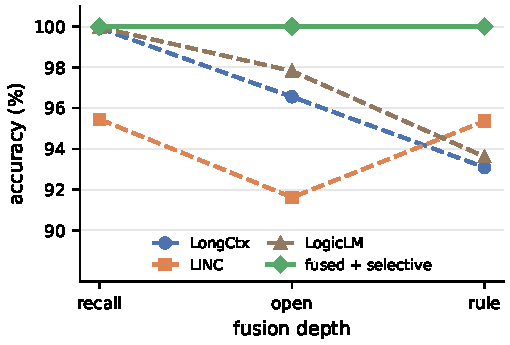
\includegraphics[width=\columnwidth]{by_type}
\caption{Accuracy against fusion depth. The lines cross. Systems that combine
evidence loosely are strong where the answer is a stated value and weak where a
rule must be applied; the system that formalises every question is the reverse.}
\label{fig:bytype}
\end{figure}

The overall column is nearly uninformative: the three published systems sit
within \SpreadOverall{} points of each other, which would ordinarily be read as
three comparable systems. Split by depth, they are not comparable at all.

LongCtx and LogicLM find stated values almost perfectly, at
\AccLongCtxRecall\% and \AccLogicLMRecall\%, and then fall to
\AccLongCtxLogic\% and \AccLogicLMLogic\% once a rule must be applied. The
evidence they need is in front of them; what fails is combining it with a
constraint that is not in the record.

LINC behaves in the opposite way. It is the strongest of the three on
rule-governed questions at \AccLINCLogic\%, which is what its design targets,
but the weakest on recall at \AccLINCRecall\% and on open questions at
\AccLINCOpen\%. Because it translates every question into a formal
representation before answering, it applies deep-fusion machinery to questions
that need none, and pays for it. Depth-three capability bought this way is not
free.

That is the finding we consider most useful: on this benchmark, being good at
one depth has come at the cost of another. The last row of Table~\ref{tab:main}
gives the headroom, the accuracy still available to the best baseline at each
depth. It rises monotonically, from \HeadroomRecall{} points at depth one to
\HeadroomOpen{} and then \HeadroomLogic{}. The remaining errors are not
retrieval errors, and they are not distributed evenly.

% AUTO-GENERATED by make_examples.py -- do not edit by hand.
% Questions, gold values and answers are read from the released result files.
\begin{table*}[t]
\caption{One worked example per question class, quoted from the released per-question outputs. A tick marks the recorded verdict; wrong answers are set in italic. None of these failures is a fluency failure: every wrong answer is well formed and plausible, and each substitutes the system's own prior for what the record states. Answers in the depth-aware column also carry the identifier of the record they were drawn from, omitted here for width. The first three rows are from the verified subset; the fourth is from a separate compositional evaluation, on which LINC was not run. That answer has three components and the systems differ on exactly one, shown in bold, so the cell lists the three components rather than the full sentence.}
\label{tab:examples}
\centering\footnotesize
\setlength{\tabcolsep}{3.5pt}
\hyphenpenalty=10000\exhyphenpenalty=10000
\begin{tabular}{@{}>{\raggedright\arraybackslash}p{0.228\textwidth}>{\raggedright\arraybackslash}p{0.134\textwidth}>{\raggedright\arraybackslash}p{0.104\textwidth}>{\raggedright\arraybackslash}p{0.134\textwidth}>{\raggedright\arraybackslash}p{0.134\textwidth}>{\raggedright\arraybackslash}p{0.142\textwidth}@{}}
\toprule
question (gold in italics) & LongCtx & LINC & LogicLM & depth-aware & verdict \\
\midrule
\textbf{basic}\newline According to viessmann\_seed\_0017, what is the Standard?\newline \textit{2 years parts \& labour} & \checkmark~2 years parts \& labour & $\times$~\emph{EU F-Gas Regulation} & \checkmark~Standard: 2 years parts \& labour & \checkmark~2 years parts \& labour & LINC swaps the declared field for a real regulation \\[3pt]
\textbf{open}\newline According to viessmann\_seed\_0002, what is the EU authorised representative?\newline \textit{Same as manufacturer} & \checkmark~Same as manufacturer (sample) & $\times$~\emph{Viessmann Climate Solutions SE} & \checkmark~Same as manufacturer (sample) & \checkmark~Same as manufacturer (sample) & LINC answers from world knowledge, not from the record \\[3pt]
\textbf{reasoning}\newline Is Gas a Thing?\newline \textit{Thing} & $\times$~\emph{no} & \checkmark~yes & $\times$~\emph{"Gas"} & \checkmark~Yes. Gas is a Thing. & both answer from plausibility rather than the schema \\[3pt]
\textbf{multi-source}\newline Using my saved preference and both product records: give my preferred supplier for ProductB, one compliance…\newline \textit{PrintPack | RoHS | separate collection symbol…} & $\times$~\emph{PrintPack $\cdot$ \textbf{UN 38.3} $\cdot$ separate collection symbol} & \textit{not run} & $\times$~\emph{PrintPack $\cdot$ \textbf{UN 38.3} $\cdot$ separate collection symbol} & \checkmark~PrintPack $\cdot$ \textbf{RoHS} $\cdot$ separate collection symbol & each recovers two of three sources, then substitutes a real but wrong standard \\[3pt]
\bottomrule
\end{tabular}
\end{table*}


Table~\ref{tab:examples} gives one worked example per class, quoted from the
released outputs. What the aggregate numbers cannot show is that none of these
failures looks like a failure. Asked what warranty standard a heating record
declares, LINC answers \emph{EU F-Gas Regulation}: a real regulation, correctly
spelled, and not what the record says. Asked who the EU authorised
representative is, it answers with the manufacturer's legal name rather than the
declared value \emph{Same as manufacturer} --- it resolved the reference instead
of reporting the field. At the reasoning class the direction reverses, and the
two systems that combine evidence loosely answer from plausibility: asked
whether \emph{Gas} is an entity in the product schema, both decline it, while
the schema itself asserts that it is.

The last row extends the pattern to a question with three sources at once: a
value the user set earlier in the session, a compliance constraint, and a field
from a passport document. Both baselines recover two of the three and then agree
on the same wrong answer, replacing the required standard with \emph{UN 38.3} ---
again a real standard, and the wrong one here. This row comes from a separate
compositional evaluation rather than the verified subset, and LINC was not run
on it; we report it as an illustration, and it contributes no number to any
table.

The common shape is that each wrong answer substitutes the system's own prior
for what the record states, and does so fluently. This is why answer-level
review does not catch these cases in practice, and why the paired design in
Section~\ref{sec:paired} matters more than the averages.

Table~\ref{tab:domain} shows this is not an artefact of one domain. Ordering the
three domains by the share of rule-governed questions they carry, from
\ShareMostRule\% down to \ShareLeastRule\%, baseline accuracy falls in the same
order. With \VerifiedDomains{} domains this is an ordering rather than a
correlation, and we report it as such.

\begin{table}[t]
\caption{Accuracy by industrial domain, ordered by the share of rule-governed questions each domain carries. Baseline accuracy falls as that share rises; the ordering is recomputed from the artifacts on every build.}
\label{tab:domain}
\centering\footnotesize
\setlength{\tabcolsep}{5pt}
\begin{tabular}{lccc}
\toprule
configuration & battery & lexmark & viessmann \\
\midrule
rule-governed share (\%) & 53.9 & 45.7 & 33.3 \\
\midrule
LongCtx & 93.70 & 96.82 & 97.75 \\
LINC & 93.77 & 92.56 & 97.60 \\
LogicLM & 94.25 & 97.56 & 97.79 \\
\midrule
fused + selective & 100.00 & 100.00 & 100.00 \\
\bottomrule
\end{tabular}
\end{table}


\subsection{Selective fusion pays no penalty here}
\label{sec:paired}
The trade-off above is what a selective strategy is meant to avoid: apply
symbolic combination to the questions that need it, and leave the others alone.
Whether that works cannot be settled by average accuracy, because a system can
improve on average while losing cases elsewhere, which is exactly what the
uniform strategies do. Since every configuration is scored on identical rows,
the comparison can be paired instead: for each question we can ask which
configurations got it right. Table~\ref{tab:mcnemar} counts the disagreements in
both directions.

\begin{table}[t]
\caption{Paired disagreement. The right-hand column is zero for every baseline:
no baseline answers correctly a question the fused configuration misses.}
\label{tab:mcnemar}
\centering\footnotesize
\setlength{\tabcolsep}{5pt}
\begin{tabular}{lcc}
\toprule
baseline & fused-only correct & baseline-only correct \\
\midrule
LongCtx & \DiscLongCtxSysOnly & \DiscLongCtxBaseOnly \\
LINC & \DiscLINCSysOnly & \DiscLINCBaseOnly \\
LogicLM & \DiscLogicLMSysOnly & \DiscLogicLMBaseOnly \\
\bottomrule
\end{tabular}
\end{table}

The baselines leave \ErrLongCtx{}, \ErrLINC{}, and \ErrLogicLM{} errors on these
rows; the selective configuration leaves \ErrSys{}. Each comparison is
significant by an exact McNemar test at $p < 10^{-\McnExp}$, but the zeros in
the right-hand column say more than the $p$-values do. Where LINC bought
rule-governed accuracy by giving up recall accuracy, applying symbolic
validation selectively gave up nothing measurable on this set. That is the
difference between a depth-aware strategy and a uniform one, and it is visible
only because the comparison is paired.

\subsection{Knowing when the sources are not enough}
Deciding whether to answer is itself a fusion question: it asks whether the
combined evidence is sufficient. To test this away from the documentation the
configuration was developed on, we evaluate \OffN{} queries over Open Food
Facts~\cite{openfoodfacts}, a public product database with different field
names, a different schema, and a great deal of genuinely missing data.

Accuracy here is \emph{decision} accuracy: answering correctly when the record
supports an answer, and staying silent when it does not. The configuration
reaches \OffAcc\% (Wilson 95\% interval \OffAccLo--\OffAccHi\%) while answering
\OffCoverage\% of queries. Its calibration error is \OffEce{} and the area under
its risk--coverage curve is \OffAurc{}. When it does stay silent it is almost
always right to: abstention precision is \OffAbstainPrec{} at recall
\OffAbstainRec{}.

\begin{table}[t]
\caption{Public-schema arm by query type. Where the underlying fields are sparsely populated there is little to combine, and the system lowers coverage rather than guessing.}
\label{tab:off}
\centering\footnotesize
\setlength{\tabcolsep}{4.5pt}
\begin{tabular}{lcccc}
\toprule
query type & $n$ & accuracy & coverage & ECE \\
\midrule
nutrition & 1450 & 100.00 & 69.6 & 0.004 \\
missingness & 367 & 92.92 & 100.0 & 0.071 \\
attribute & 1146 & 99.83 & 99.8 & 0.002 \\
sustainability & 1039 & 91.92 & 38.0 & 0.060 \\
fairness & 19 & 100.00 & 100.0 & 0.000 \\
\midrule
all & 4021 & 97.21 & 73.0 & 0.021 \\
\bottomrule
\end{tabular}
\end{table}


Table~\ref{tab:off} shows the behaviour is not uniform across the \OffTypes{}
query types. Questions about stated nutrition values and product attributes are
answered essentially perfectly, which is depth one on a new schema. The hardest
type is \OffHardestType{}, at \OffHardestAcc\%, and there the system answers
only \OffHardestCoverage\% of the time. Those fields are sparsely populated and
inconsistently defined across the database, so there is often little to combine,
and the system responds by declining rather than guessing. Its calibration error
rises on the same slice, to \OffEceHardest{}, which is the behaviour we want: it
is least confident exactly where it answers least often.

% =====================================================================
\section{What This Shows, and What It Does Not}
\label{sec:limits}
% =====================================================================
A perfect score invites suspicion, and it should. Four qualifications matter.

The trade-off is observed across three published systems on one benchmark. It is
a real property of those systems on these questions, and the direction is what
their designs predict, but three points do not establish that every uniform
strategy must pay this cost. The claim we defend is the weaker one: reporting a
single accuracy figure would have hidden a difference that matters for choosing
between them.

The separation at depth three is concentrated, and we would rather state where
than have it found. \ScopeNarrow{} of the \NLogic{} schema-governed questions
ask about the schema vocabulary rather than product content; excluding them
raises the baselines to \CleanLongCtxLogic\%, \CleanLINCLogic\% and
\CleanLogicLMLogic\% there, and the headroom no longer rises monotonically. On
that subset the baselines return a fixed premise list, consistent with the
vocabulary never reaching their context, so part of the gap is an information
difference rather than a reasoning one. Separately, a refusal is scored as a
wrong answer, which accounts for \AbstainShareLINC\% of LINC's errors. The
released code reports all three, and the result that survives every re-grading
is the zero in Table~\ref{tab:mcnemar}.

The verified set is, by construction, the set of questions with unambiguous
answers, and its rule-governed part is checked against machine-readable
constraints. A configuration that routes those questions to that check is
expected to reach the ceiling. The result shows the ceiling is reachable and
that the baselines do not reach it; it says nothing about the questions the set
excludes. Those \ExcludedRows{} rows are published so that this boundary can be
inspected rather than taken on trust.

The one-sided result holds for these rows. It shows that on this benchmark the
improvement costs nothing, but zero disagreements in \VerifiedN{} paired
comparisons is not a guarantee about unseen questions.

The two arms measure different things and should not be averaged. The verified
set measures accuracy where an answer exists. The public-database arm measures
whether the system knows when one does not, which is why coverage and
calibration are reported there. Whether \OffCoverage\% coverage is acceptable
depends on what a withheld answer costs in a given setting.

Finally, this paper compares configurations. It does not attribute the
difference to any single mechanism; separating the contribution of symbolic
validation from that of selective abstention requires an ablation, reported
separately.

% =====================================================================
\section{Conclusion}
% =====================================================================
Grouping questions by how many sources an answer must combine changes what the
numbers say. A single accuracy figure puts three published systems within
\SpreadOverall{} points of each other. Split by fusion depth, the ordering
inverts: the system that formalises every question leads on rule-governed
questions and trails everywhere else, while the systems that combine evidence
loosely do the reverse. Reporting one number per system hides a trade-off that
determines which system a practitioner should actually choose.

For product-passport records this has a direct consequence. Locating a stated
value is effectively solved, so further work on retrieval has little left to
recover; the available accuracy is concentrated at the depth where a retrieved
value must meet the schema that classifies it. But buying that depth uniformly, by pushing
every question through a formal representation, costs accuracy on the questions
that never needed it. Applying validation selectively, and withholding an answer
when the combined evidence is insufficient, closed the gap on our verified set
without costing accuracy anywhere on it.

The domain here is product passports, whose records are schema-bound by
construction, which is what makes the deepest level common. But nothing in the
analysis is specific to them. Any setting where answers must combine stored
records with a schema or rule base held separately from those records ---
clinical coding, financial reporting, safety certification --- should expect the
same shape, and is better served by measuring fusion depth than by reporting a
single accuracy figure. Whether the pattern extends to genuinely
threshold-governed compliance questions, which this benchmark does not contain,
is open.

\section*{Reproducibility}
The verified set, its exclusion records with reasons, the per-question outputs
of all four configurations, and the public-database evaluation summary are
released at \url{https://github.com/aeturzo/dpp-qa-fusion-depth}. Every number in
this paper is generated from those files, and the released
\texttt{verify\_all.py} re-derives all of them and fails if any disagrees with
the value printed here; none is transcribed by hand. The same repository
reports what changes under stricter grading of the question classes.

\section*{Acknowledgment}
This work was supported by the CE-RISE project, which has received funding from
the European Union's Horizon Europe research and innovation programme under
grant agreement No.\ 101092281. Views and opinions expressed are those of the
authors only and do not necessarily reflect those of the European Union or the
granting authority, neither of which can be held responsible for them.

\section*{Generative AI Disclosure}
Generative AI assistants (Anthropic Claude; OpenAI Codex) were used for language
editing, \LaTeX{} preparation, and the reproducibility tooling released with this
paper. They were not used to produce, select, or analyse experimental results:
every figure reported here is generated from locked evaluation artifacts by the
released scripts. The authors verified every claim, reference, and numerical
value against those artifacts and are solely responsible for the content.

\bibliographystyle{IEEEtran}
\bibliography{refs}

\end{document}
